%% Template for SDP report, adapted from mlp_cw2_template, 2018. 

%% Based on  LaTeX template for ICML 2017 - example_paper.tex at 
%%  https://2017.icml.cc/Conferences/2017/StyleAuthorInstructions

\documentclass{article}
\usepackage[T1]{fontenc}
\usepackage{amssymb,amsmath}
\usepackage{txfonts}
\usepackage{microtype}
\usepackage{xspace}
\xspaceaddexceptions{\%}

% Lists with less spacing between items
\usepackage{paralist}

% For figures
\usepackage{graphicx}
\usepackage{subfig} 

% For citations
\usepackage{natbib}

% For algorithms
\usepackage{algorithm}
\usepackage{algorithmic}

% the hyperref package is used to produce hyperlinks in the
% resulting PDF.  If this breaks your system, please commend out the
% following usepackage line and replace \usepackage{mlp2017} with
% \usepackage[nohyperref]{mlp2017} below.
\usepackage{hyperref}
\usepackage{url}
\urlstyle{same}

% Packages hyperref and algorithmic misbehave sometimes.  We can fix
% this with the following command.
\newcommand{\theHalgorithm}{\arabic{algorithm}}


% Set up MLP coursework style (based on ICML style)
\usepackage{mlp2018}
\mlptitlerunning{SDP Demo \demoNumber  Group (\groupNumber)}
\bibliographystyle{icml2017}


\DeclareMathOperator{\softmax}{softmax}
\DeclareMathOperator{\sigmoid}{sigmoid}
\DeclareMathOperator{\sgn}{sgn}
\DeclareMathOperator{\relu}{relu}
\DeclareMathOperator{\lrelu}{lrelu}
\DeclareMathOperator{\elu}{elu}
\DeclareMathOperator{\selu}{selu}
\DeclareMathOperator{\maxout}{maxout}






\usepackage{rotating}
%% You probably do not need to change anything above this comment

%% REPLACE the details in the following commands with your details
\setGroupNumber{22}
\setGroupName{The Two-Twos}
\setProductName{PlantED}
\setLogoFileName{figs/plantED_logo.png}

\begin{document} 

\makeSDPTitle{Project Plan}

% Previous MLP Style Title Layout working. 
% \twocolumn[
    % \mlptitle{\productName: SDP Demo \demoNumber}
    % \centerline{Group \groupNumber: \groupName}
% ]

\begin{abstract} 
% PlantEd is a smart plant care system allowing beginner plant enthusiasts to grow their plants while also learning the optimal conditions for growth.

% Plants will grow inside a modified propagator in which we have implemented all the features fundamental to plant growth such as: water, sunlight, temperature and soil. We will also be implementing additional features to enhance user experience such as motion capture of the plant as it grows. All of these features will be accessible through our web app which will allow users to: monitor the growing environment, change the environment (i.e change variables as they please such as moisture) and learn the necessary plant-care skills.

PlantEd is a smart plant care system that intends to enhance the learning curve of new plant enthusiasts by providing an interactive experience for growing plants indoors, and by assessing the optimal conditions for growth.

Plants can be grown inside the modified propagator system, which monitors the conditions fundamental to plant growth: water, sunlight, temperature, humidity and soil pH. To provide a rounded and educational experience, the system implements modes of automatically altering the aforementioned conditions. For example, to control exposure to sunlight and ensure that the plants grow upright the propagator will be able to adjust its position to control the effects of phototropism.

This system will be accompanied by a website application that allows users to track the conditions of the plants, and to alter environmental factors as desired. This website will provide useful information for beginners about various plant species, and to further enhance user experience we intend to implement features such as stop-motion which will allow users to capture the growth journey of their plants.

\end{abstract} 

\section{Pitch} 

The COVID-19 pandemic has resulted in a dramatic rise in the popularity of owning and caring for plants, however 48\% of people surveyed admit to being anxious about how exactly to keep plants alive and healthy - to the extent where the average 'plant parent' has killed 7 houseplants (hou, 2020). %\cite{houseplantsurvey}

To manage these inhibitions, we propose PlantED - a plant care system geared towards beginners with an interest in learning about growing and caring for plants. We understand that the learning curve here can be daunting, with many aspects of plant-care taking time and experience to master, so our goal is to provide an experience where users get to grow plants themselves, with help from our system and helpful information to aid learning.

By developing an assistive plant-care system from a beginner-friendly perspective, we aim to gradually introduce users to the various factors that contribute to growth. This will be done by isolating different skills, for example watering and light management, in a way that allows a user to take control of these dimensions as and when desired. 

In addition to being an assistive learning tool, the development of this product also serves to have a positive impact on the surrounding people and environment. In particular, the fact that the plant care system will help take care of your plants when you are away ensures that the indoor air pollution is reduced. There has been research that shows that 4 million people worldwide die prematurely due to indoor air pollution and counteracting this is a main concern (RHS, 2021a). Moreover, encouraging more people to become involved in planting should introduce the benefits of enhanced concentration, learning performance and memory retention that arise from plants being in the vicinity(A&M) %\cite{Ellison}. 

Furthermore, there are a lot of plants that are extremely difficult to grow since they require a great deal of attention and specific conditions such as Orchids (Middleton, 2018), PlantED solves this issue by taking care of peoples' plants whilst teaching them the necessary education for plant growth. 
%Figure \ref{fig:proto} shows


% %
% \begin{itemize}
%   \item Moreover, it has a potential educational value as students today are reluctant to learn about plants. This could provide a more fun way of engaging/introducing how to take care of plants. Making learning about plants more engaging can reduce the plant blindness that is emerging. \cite{plantsbooklet, ppparticle}
%   \item Discuss the importance of having plants in the vicinity and the impact it has on both the environment and the people. In addition, to just being instructional can take care of your plant when you are away, which would otherwise make it hard to capitalise on the benefits of plants [4 (this one is about effect on learning performance), 5 (this one is about enhanced accuracy, concentration, retention etc that is caused by the calming environment)]
%   \item Research has shown that 4 million people worldwide die prematurely due to indoor air pollution and by supporting/encouraging the people that want to get into planting we are attempting to counteracting this phenomenon (the contamination can cause Sick Building Syndrome). Note that although opening the windows does help, it has been recorded that during winter periods the contamination is relatively large due to the windows being open less. [6]
%   \item There are many plants which are extremely difficult to grow as they require a lot of attention and specific conditions that the average person can't provide. For examples Orchids need to be between 15 to 30 degrees, prefer shade during the day and must allow soil to dry before watering again[8]. PlantEd solves this issues allowing the average person to grow all plants even those that require intense care.
%   \item There aren't many products that do sun tracking on the market which will help our product stand out.
%   \item We have identified a gap in the market as we have discovered a new target group for plant care, those people who are plant enthusiasts or people who want to learn more about plant growth. Previous robotics systems in this sector focused heavily on individuals who merely care about having a robot water their plant and for industrial purposes.
%   \item Learning curve for beginner gardeners / growers can be very steep with many different aspects of plant-care needed to be mastered. A more beginner-friendly approach could isolate certain skills such as watering or light management to allow beginners to learn quicker and see good results from day one.
%   \item Environmental advantages - growing vegetables at home / school has no food miles.
%   \item A great tool for schools (of all ages) as we can adapt the User experience to suit the age of the user. It will also give pupils a chance to escape the sometimes mundane written classes and get hands on with plants.
%   \item Good for schools or homes in urban areas or inhospitable climates where access to areas for plant growth is very limited.
%   \item Allows for growth of more exotic plants that wouldn't be grow-able otherwise outdoors, good educational potential.
%   \item To augment and not to overly-automate the plant growing process.
%   \item Indoor drying is not good for health. People need to use the air humidifier to humidify the air. Our product can replace that machine by cultivating particular plant species. Our products not only naturally increase indoor humidity, but also reduce electricity use to respond to climate change.
%   \item A great product for improving mental health. Gardening or planting can mitigate people's stress and depression.
%   \item Our product helps teenagers to change the focus from social media to nature.
  
% \end{itemize}

% 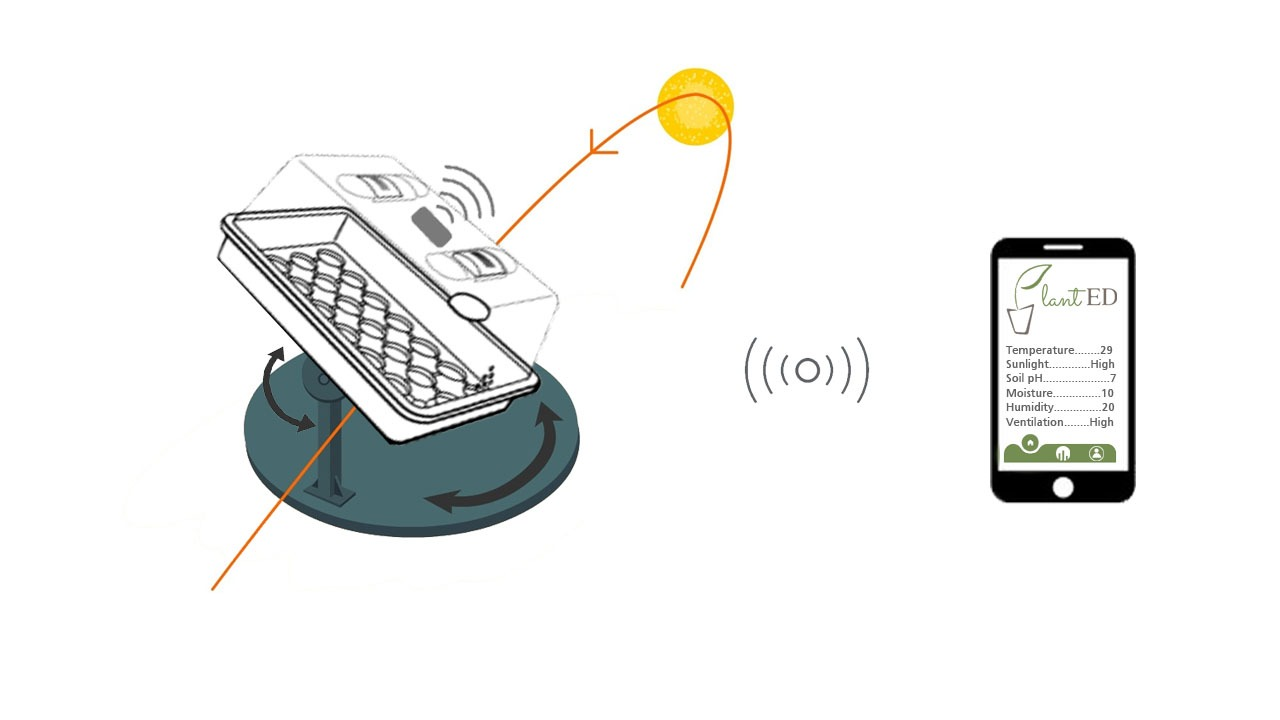
\includegraphics[width=0.55\textwidth, inner]{figs/proto.jpg}

\begin{figure}[h]
\vskip 5mm
\begin{center}
\centerline{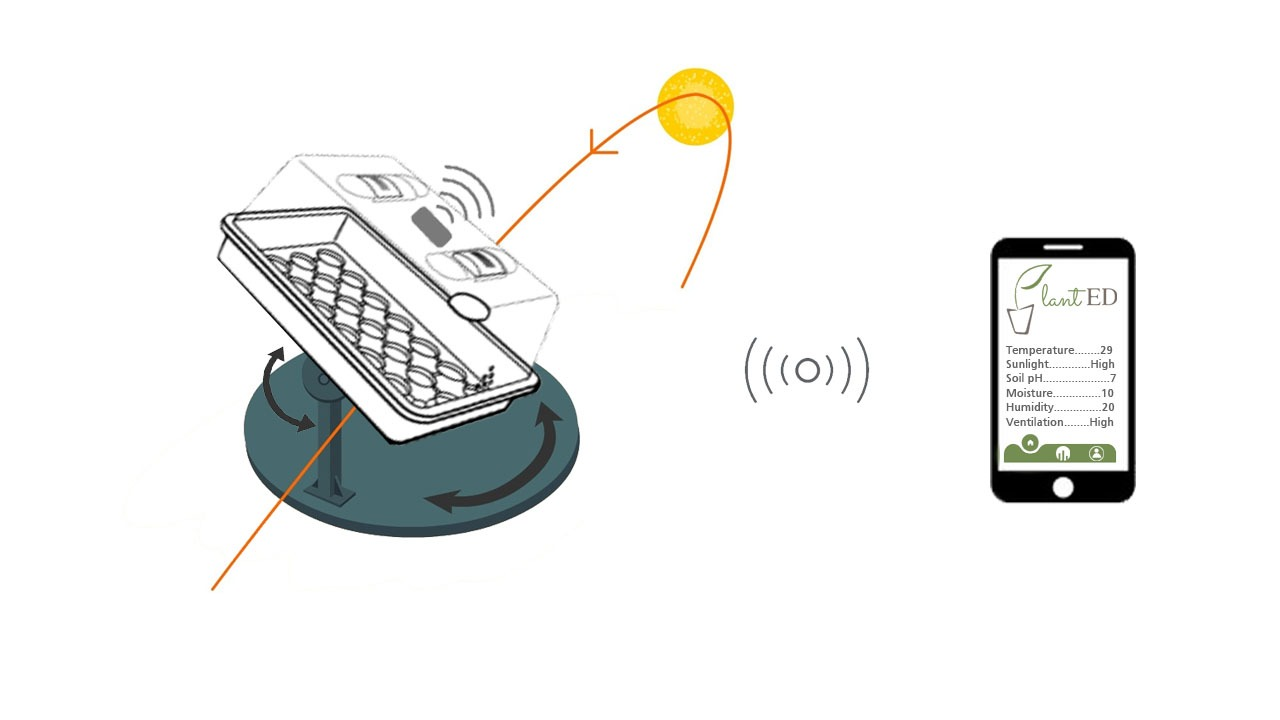
\includegraphics[width=\columnwidth]{figs/proto.jpg}}
\caption{An illustration of the system.}
\label{fig:proto}
\end{center}
\vskip -5mm
\end{figure} 


\begin{figure}[h]
\vskip 5mm
\begin{center}
\centerline{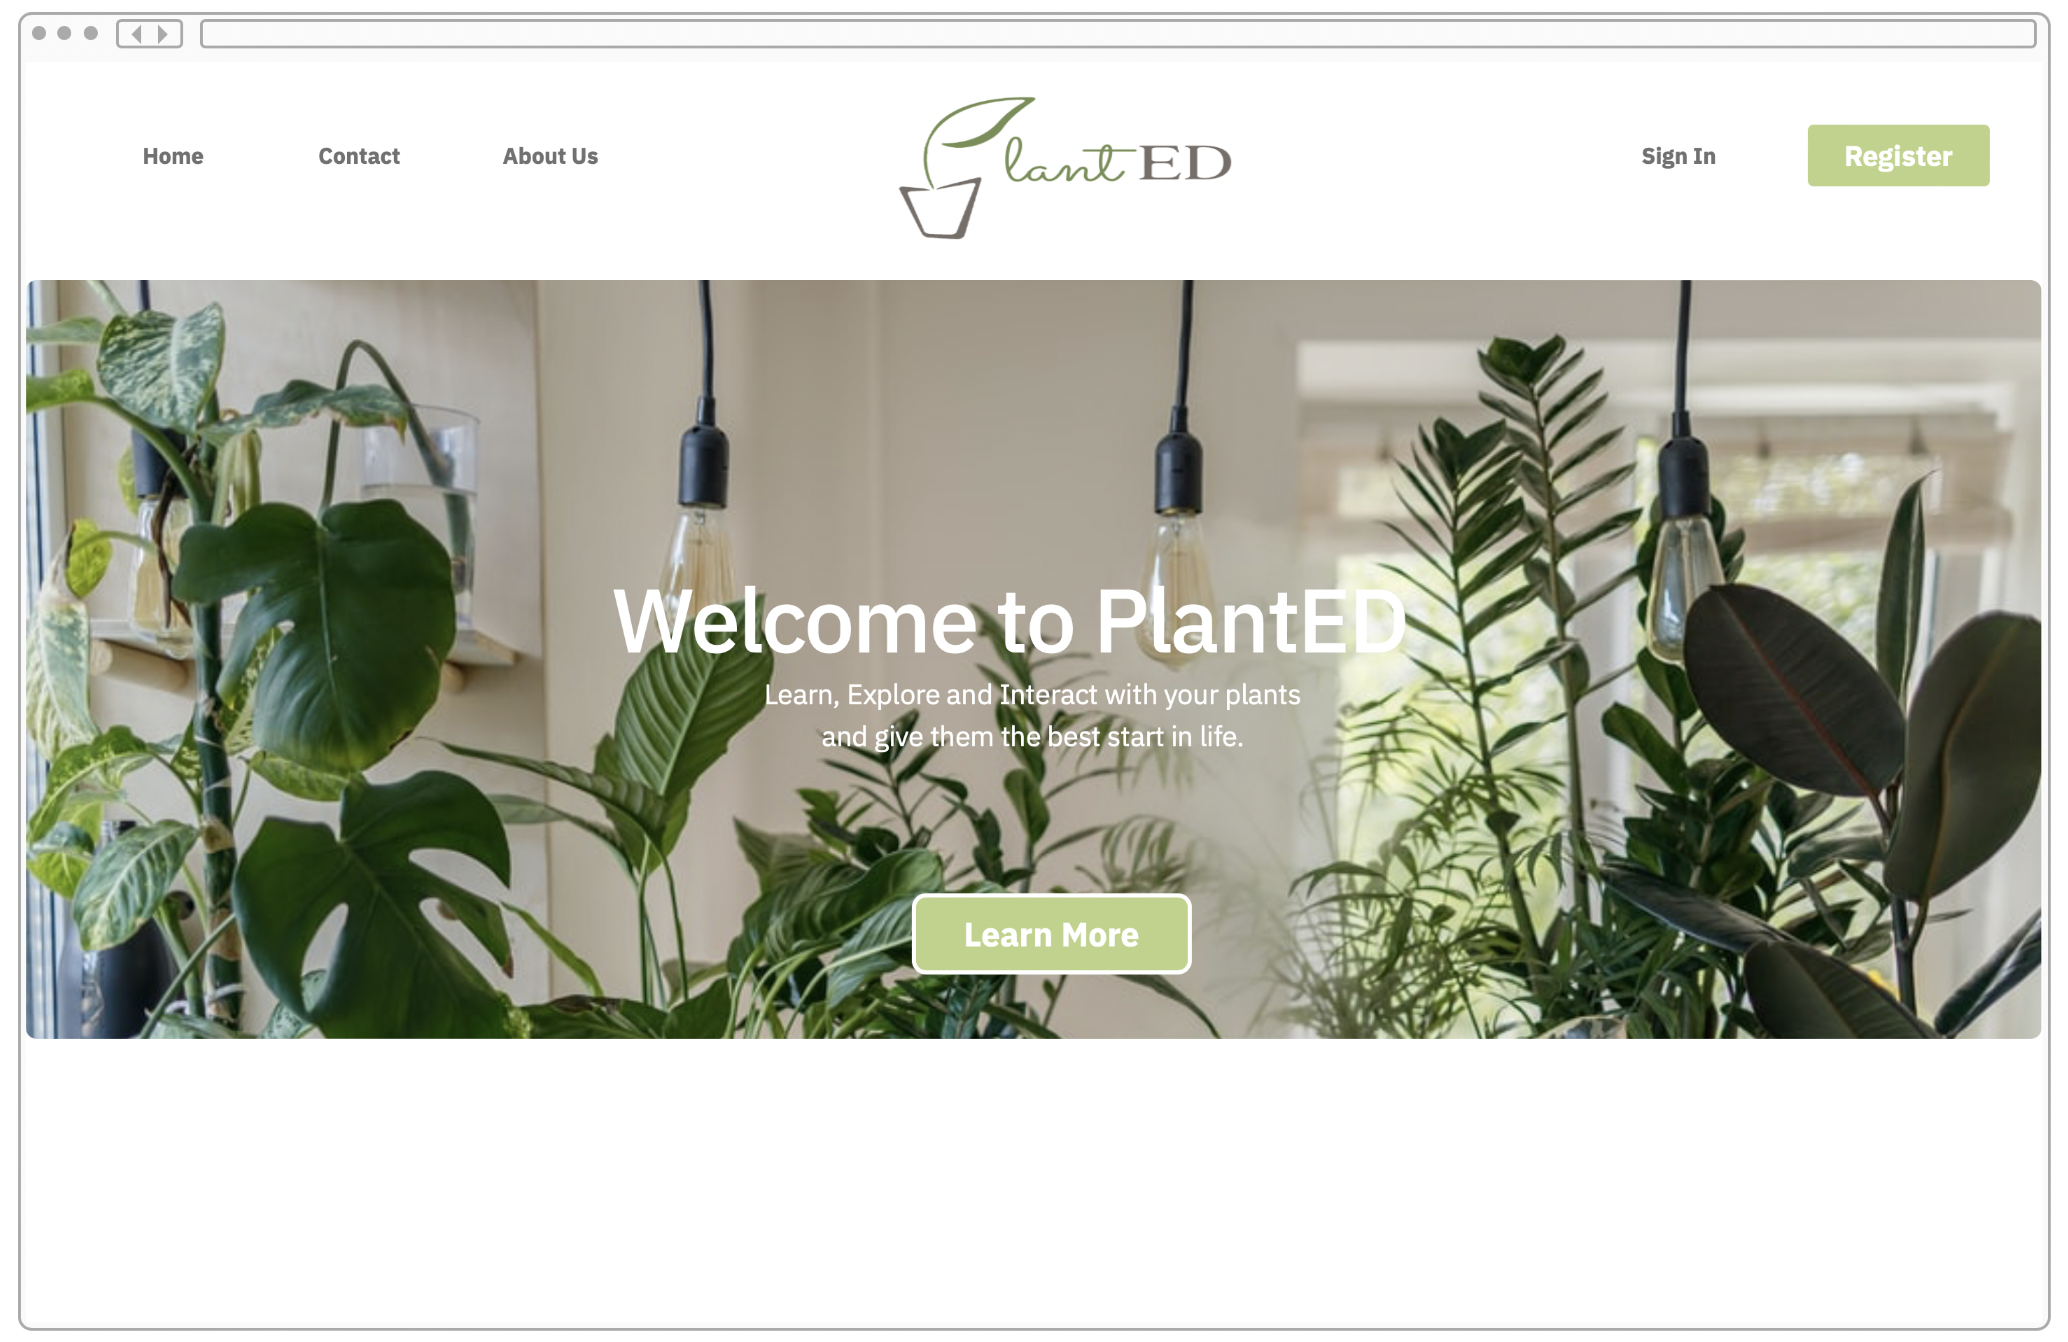
\includegraphics[width=\columnwidth]{figs/homepage_mockup.png}}
\caption{UI mock up for website application homepage.}
\label{fig:app}
\end{center}
\vskip -5mm
\end{figure}

\section{The Team}

\subsection{Overview}
The team consists of nine diverse people that have relevant competence in both the hardware and software aspects of the project.

\subsection{Working Preferences}
The interdisciplinary nature of the project means that there are different working preferences such as work- intensity and hours. Nonetheless, the team would overall want to ensure an evenly spaced workload throughout the whole project timeline.

\subsection{Members}
\subsubsection{Eric Gallagher}
From completing several courses in business Eric has developed a strong skill set in marketing, which makes him well suited for tasks involving pitching and commercialisation. In addition to this he is a proficient programmer so will be involved with the software components of the project however he has little experience in robotics. He plans to deal with this weakness by continuous collaboration with the hardware department.

\subsubsection{Casey Gong}
Casey will be supporting the team on the software side in particular front-end development with her extensive knowledge of app development. In fact, she recently finished an IOS application development course, giving her confidence in building an application through collaboration. She has some experience in website development using HTML, CSS and JavaScript. Moreover, she is also interested in machine learning using online libraries such as pandas, as well as attempting to implement computer vision functionalities if there is space for extensions. Her main weaknesses lie in the robotics field, but also in interfacing hardware with software such as the use of Raspberry Pi. However, she sees this as an opportunity to learn more about these aspects.

\subsubsection{Susanna Lassila}
Susanna has relevant marketing skills due to a recent business course and some experience in web-development. However, she is more interested in working with the hardware side of things as she would like to gain more knowledge and experience in that area. She suspects that she might struggle with learning these skills, however despite this area being one of her weaknesses she is enthusiastic about dealing with this challenge as she wants to learn new things.

\subsubsection{Dafydd Foster Evans}
Dafydd has experience in using and implementing certain hardware technologies such as the Raspberry Pi, ROS and Arduino. He has used them during his degree for various projects. In addition, he has had some experience in creating small start-ups such as this one and hopes to bring some of this experience into the group. His strong experience in the hardware side comes at the cost of less experience in software related tasks such as web and mobile applications, but he is confident that this can be overcome with collaboration.

\subsubsection{Fadi Barazi}
Fadi has strong expertise in both hardware and software from designing very low level hardware components such as printed circuit board using tools such as kiCAD to programming FPGAs using HDLs such as Verilog, but also using C. In addition, he developed a particular interest into machine learning and software. This combination of both hardware and software has enhanced his passion to learn more about interfacing hardware with software during this project. He has not been involved in large team projects before and so he suspects that he might struggle with the teamwork aspect, but he sees this as a valuable experience for the future.

\subsubsection{Oscar Alberigo}
The courses that Oscar has taken during his University degree have made him proficient in programming applications in React Native (based on JavaScript) and developing apps for both iOS and Android. In one of his recent projects, he has had to grasp the skills of using Firebase for authentication and databases to store user information. Oscar is in particular looking forward to bridging the gap between software and hardware as this is his first interaction with hardware pieces. He has also not been involved with large scale projects and has relatively little knowledge on how to receive outputs from I/O hardware and thus it might be a challenge to grasp this understanding in the relatively little time we have, however jumping into these new problems could provide a great learning curve for him.

\subsubsection{Ananya Majumdar}
Ananya has experience working in Agile workflows to design and implement systems dealing with heavy and constant flows of data and so she would be able to contribute to the development of the software processing and storing the data that will be received from various hardware components. She has also previously worked with some of the hardware platforms that are readily available to us so this puts her in a good position to contribute to this interface between hardware and digital information. However, Ananya does struggle with planning and maintaining schedules for mid-to-large sized projects, which is the motivation behind her positioning as project manager as this will serve as a learning experience.

\subsubsection{Binbin Zhan}
 Binbin has had experience in 3D-modelling and UI design for product product web- and mobile-applications, which is the area that he is keen to work on. In additon, he is adept at constructing simulations and cartoons that can be used during the marketing phase of the product. Furthermore, his main weakness lies in dealing with robotics both on a hardware and software level, but he is confident that he will be able to overcome this.

\subsubsection{Bohan Xu}
Bohan has experience in web design and especially HTML, CSS and JavaScript. He is interested in machine learning and has some knowledge about deep learning and so he would want to work on the data processing side of things. However, he is mostly interested in the middle-ware part such as ROS and would like to deal with it if incorporated into the project. He has no experience and knowledge with ROS and hardware, but he is adept at dealing with challenges and so is optimistic. In addition, has had similar team projects before and so is confident in his teamwork abilities.


\section{Users} 
% \begin{itemize}
%     \item Main target audience are for individuals that want to get into planting but have no proper experience or guides to how they would start. The intention is also that this device could potentially be incorporated in the educational sector to aid teaching in schools.
%     \item The intention is that the device provides a more interesting interaction when getting involved with plants, enhancing the user understanding of plants in a shorter time by allowing them to engage directly with the task instead of just reading a bunch of books etc.
%     \item However, issue with this design might be that not everyone can utilise it such as the visually impaired. Moreover, there will be some mobile-app functionalities, which older individuals might be reluctant to use as they might not have that technical competence.
%     \item Design considerations to avoid being noisy and disturbing.
%     \item Electricity supply considerations - whether its safe to charge it from home socket.
%     \item Design considerations to allow freedom of users to water / shifting positions of the device themselves. But reminders could be sent to them for doing something faulty. 
%     \item Design considerations for users with no gardens. Might have indoor substitution features for indoor users.
%     \item The gadget will (most likely) be used at home/office and so co-workers, family members or even just maintenance people might interact with it. For these individuals, the focus is most likely not going to be based on the the effectiveness of the device to help in understanding how to treat plants, but more so the noise that it produces, the space it occupies, the ornamental nature of device and even how easily it can be cleaned. These things should be considered to ensure inclusiveness and consideration of the surrounding people.
%     \item Although this device might also to some extent be used by the educational sector, it might be the case that their needs are more sophisticated (such as being able to observe more variables or investigate the plant on an anatomy level) than the normal user that wants to get into planting, which the device will not be able to fully provide. This should be considered in marketing.
%     \item Might be important to consider how the UI or usability should change when used by parents / teachers vs by children / students. Might be useful to have a parent portal that can change certain settings behind the scene, and simplify some of the features for younger (or less experienced) users.
%     \item Installation team is not the primary user but it has to make sure sun tracking component of the device does not let it go beyond gardens and help the users figure out solution with charging the device.
%     \item Older people might not be targeted because there is low mobile phone usage rate, unfamiliarity with new technology and relatively lower learning speed. Many of them would want to completely take care of plants themselves rather than using robotics since they generally have more leisure time.
%     \item Other stakeholders:
%     1.surrounding people  - neighbourhood,campus
%     2.Electricity suppliers - does charging of large device in households obey rules of electricity suppliers
    
%     \item Design consideration to allow users manually replacing broken sensors.
%     \item Another target audiences are for people who work a lot and do not have enough time on planting. Our product can remind them to or automatically water the plant. Target audiences can get a breath during busy work and enjoy a peaceful moment.
%     \item Scientists might be a potential target. Once our product can successfully cultivate all plants, they will consider the feasibility of large-scale indoor farming.
    
% \end{itemize}

\subsection{Main Target Audience}
The main target audience would be individuals interested in growing plants that but lack the necessary experience and knowledge to do so successfully. Hence, the intention is for the device to provide a more interesting interaction when starting to get involved with plants, enhancing the user's understanding of plants in a shorter time by allowing them to engage with the planting activities as they receive guidance from the smart plant care device. This would be done through the use of a website application that would support and guide the user during the early stages of their plant growth. In addition, there will be robotic hardware features such as light-adjustment and plant watering that will allow the user to observe how a plant should be treated. In creating a more light-hearted and engaging plant-care experience, the user should become less anxious and enjoy the process.

\subsection{Target Audience Issues}
The main challenge in designing the smart plant care device resides in the consideration of the different needs of the target audience. A lot of people interested in plant growth are of the older generation (S., Danya, 2017) and these could have certain disabilities such as being less agile, visually impaired or not accustomed to new technologies. Unless these factors are considered, the product would become less accessible to disabled people and older people will be reluctant to using our technology. 

\subsection{Non-Primary Users}
The smart plant device is intended to be used in home and work environments so it is likely that individuals that have not bought the device will interact with it on a regular basis such as co-workers, family members or even just maintenance people. For these individuals, the focus will not be based on the effectiveness of the device to help in understanding how to treat plants, but more so on the noise that it produces, the space it occupies, the ornamental nature of the device and even how easily it can be cleaned. Consequently, it can clearly be seen that there is a conflict of interest between the main target audience and the non-primary users. Despite the main target audience being the focus of attention, the non-primary users' needs still have to be taken into account as from an ethical standpoint the device should not harm other individuals in order to provide value to a certain subgroup of the population. Moreover, if the non-primary users' interests are not considered the construction of the device would in some sense create another societal problem despite providing a solution for another one.

It should be emphasised that the intention is also for this device to be incorporated into the education sector to aid teaching in schools, which makes educational institutions another target audience to consider. Hence, it should be noted that their needs might be more sophisticated as opposed to the normal user that wants to learn about planting (Society of Biology, 2010). For instance, educational institutions might want the smart plant care device to be able to monitor more variables or even give some insight into the plant anatomy, which the device will not be able to fully provide. This should be made clear during the marketing phase, such that there is no misconception.

\subsection{Consideration for Non-Primary Users}
There have been considerations made to address the potential conflicts of interests between different user groups in order to ensure that a well-rounded product is constructed. First of all, there will be considerations made for how the UI and the usability of the website application should change when used by different subgroups within our target group. For instance, the User Interface for a parent and a teacher might be quite different than for children and older people. Consequently, it might be useful to have a parent portal that has certain additional settings and that some features are more simplified for the less experienced or younger user. Moreover, design considerations will be made to allow freedom to the user to decide if they would like to water the plant themselves or not. This ensures that the interests of the people that like the leisure of doing this task themselves to learn about it and the people that would want a more automated assistive gadget are both considered. Nonetheless, the intention is still to send reminders to the users that perform the task themselves if it is discovered that they have done something incorrect.


\section{Impact}
% \begin{itemize}

%     \item Main intention is to sell the system to the public since it should be accessible to anyone that wants to learn about growing plants (correct me if I am wrong)
%     \item The most significant social impact should be an enhanced learning in plant care, which should (hopefully) reduce the anxiousness of owning plants and the plant blindness that is increasing in the society of today.
%     \item raise awareness of global warming through cultivating people's interests in growing plants themselves which combats global warming.
%     \item Better air quality and better views in neighbourhood.
%     \item Might also be a useful device that enhances teaching as it creates a more engaging interaction than reading about plants and it the removes burden of having to prepare plant environments in advance from teachers.
%     \item This product would also benefit school teachers who are looking to diversify their teaching and also would provide benefits to the teacher themselves as they can have a break from teaching from a textbook and get hands on with our product.
%     \item Supporting people that want to learn about planting should hopefully also result in the adoption of more in door plants (due to the enhanced understanding of treating plants), which should reduce the effect of indoor pollution on people's health.
%     \item Moreover, the prospect of an increased adoption of in doors plants (or also a consequence of the robot keeping your plant alive while you are away) should also help in improving productivity, concentration and even memory retention.
%     \item The device should try and have a balanced effect on the users - not making them feel as if they are being replaced or surplus to requirements but that the machine is helping them grow the plant themselves. It augments not automates the process. 
%     \item If the product is cheap enough it could have the impact of democratising gardening and make it much more accessible (at least financially). Generally, gardeners are a richer, older, and more suburban subset of the population as it requires a garden [7]. The average Brit spends roughly £30,000 over their lifetime on gardening / plant care.
%     \item If we want to maximise our profit from the commercial view, I hope this system is sold to the large organization or company for educational use. We provide both hardware and software and might customise the product and make slight change following the requirement from customers.
%     \item My idea is that this product can make more people get to know the mystery of the plant grow, and inspire more people have more interest in planting and realise the green plant is an important part for the earth somehow. I think our product contributes for the environment protection.
%     \item If our product is widely used in the world, the database of our product may have a variety of plant culture data. This data can be used for educated purposes. In the university, lecturers in agricultural class can access our data, and teach students about the growth rhythm of certain species. In primary or middle school, the teacher can access our data to tell students to identify plants.
%     \item Once our product is widely used, we can notify the users and try replacing plants with crops. If this trail of indoor growth succeeded, this product could bring hope to those countries which faced food shortages.
%     \item Our product has an intelligent system to monitor the growth of plants. We can apply this system for the software patent. (We may also apply the patent design?) If we have licences, licencing to large companies can bring extra income. Investors and we both benefit from this product.


% \end{itemize}

\subsection{Product Deployment}
The main intention is to produce a system that can be sold to the public. As such it should be accessible to anyone that has developed an eagerness to learn about growing plants. In addition to the public, the product will be sold to large organisations in the education sector such as schools to be used to enhance teaching. This furthers our goal to support and encourage the learning of plant care. In order to achieve this objective, it is important to bear in mind that the product must be economically viable for a large portion of the population and not just accessible to wealthier individuals. This is an important consideration as the product should not exacerbate existing inequalities in gardening related to wealth, resulting in a negative impact.

\subsection{Potential Social Impacts}

\subsubsection{Positive Impact}

The most significant social impact should be an enhanced learning in plant care, which should hopefully reduce the anxiousness of owning plants and improve the overall interest in plants which is fading in our current society. Moreover, since the product could potentially be incorporated into education it is probable that the more engaging interaction with plants will enhance teaching as it allows teachers to diversify their teaching material (Society of Biology, 2010; Sayan and Mertoğlu, 2020). In addition, this incorporation should also reduce the burden of preparing plant environments beforehand and ensuring that these are continuously monitored. Furthermore, it should be noted that the adoption of more indoor plants should  hopefully increase, which is important as this will reduce the air pollution and as a consequence the negative impact this has on people’s health (RHS, 2021a). Note that the increased adoption of indoor plants should also contribute to a productive environment that promotes good concentration (AM; Han 2008), enhancing the overall contribution of people to society. In allowing people to explore and care for plants, there is also a likelihood of them becoming more interested in environmental aspects such as protecting natural habitats and important plant species. In addition, if the product becomes globally adopted then the database of the product will contain a variety of plant culture data, which could be used for educational purposes to teach about the growth rhythm of certain species.

\subsubsection{Negative Impact}
The smart plant care device might introduce some negative impacts and it is important to be aware of them if they are to be counteracted. First of all, the device should ensure that there is a balanced distribution in terms of plant care responsibilities between it and the user such that the user does not feel as if they have been replaced. Consequently, it is important to bear in mind that some users might want to do more work than others and the device should augment the process for these individuals and not automate it. In addition, it should be once again emphasised that the cost-effectiveness of the design is important to ensure the inclusiveness of the wider public. Generally, gardeners are a richer, older and more suburban subset of the population (S., Danya, 2017) due to the access to a garden being important and if the design is not economically viable to others then this stereotype would be strengthened. Consequently, in constructing a cost-effective solution to this problem it could turn this potential negative impact into a positive one as it would democratise and make gardening much more accessible.
 
\section{Outcomes}
% \begin{itemize}
%  \item An outcome we aim to achieve is the sunlight tracking. This will be achieved with 2 rotating axes which will use a sensor to track the sun and rotate the propagator to maximise sunlight for the plant. This is an key feature as it is necessary for plant growth.

% \item An outcome we aim to achieve is to have an app interface. We will have an app which will allow the user to interact with the care system. The app will be able to receive inputs from the system (soil pH, moisture etc) and will also be able to output to the system(temperature, water etc). 

% \item An outcome we aim to achieve is a watering system. This feature will when instructed water the plant sufficiently.

% \item An outcome we aim to achieve is ensure the system is user friendly. This means that as our target market is likely to be less familiar with technology (i.e older people or young school kids) it is essential we achieve simplicity in the design so that all can use it. The only difficulty around this outcome is measuring its success as user friendliness is not a quantitative measure however we can overcome this by running focus groups and observe how easily users are able to operate the system.

% \item An outcome we aim to achieve is temperature control. This is a another key variable for plant growth so it is essential we are able to control this variable

% \item Ideally, if we were to give the device to a genuine beginner they would be able to learn how to grow plants and successfully grow a seedling.

% \item An outcome 

% \item An outcome we aim to achieve is to swap in new components (like sensors) without having to dismantle the machine.

% \end{itemize}

The desired outcomes for the product are dependent on the fundamental objective of being able to support people as they transition into a plant care routine, which means that the concrete implementation of the system should contribute to this objective.

\subsection{Hardware Functions}
In order to support peoples' learning of different plant needs, the hardware must be designed such that it fulfills certain requirements. For instance, it is intended that the sun-tracking feature is implemented with the help of sensors such that a two-way rotating axis will rotate the plant to maximise the sunlight received based on the light required for the specific plant. In doing this, the users can observe the amount of lighting that plants require and the effect that different light conditions might have on them in terms of growth direction and speed, which would emphasize a more engaging and visual interaction to enhance the user’s rate of learning. Moreover, there will also be a watering system implemented, which when instructed will water the plant sufficiently. This feature will serve two main points, the first one being that the user will learn the amount of water that a plant might need, and the second one being that the user has a helping hand in the responsibilities of growing the plant if they are not able to do it them themselves. This is important as in addition to being a learning device, it should ensure that the user does not feel overwhelmed by all the tasks of plant care and that the device can pick up the slack when the user forgets or otherwise does not care for the plants. Furthermore, the hardware implementation will also ensure that all the relevant sensors such as soil pH, moisture, temperature, humidity, and camera are incorporated such that the user can observe the conditions that allow a plant to grow, and this would be available through the software-interface.

\subsection{Software Functions}
The hardware implementations should be accompanied by a user interface that augments the experience and allows for a user-friendly interaction. The intention is to have a website application interface that will allow the user to interact with the plant care system. The website application will be able to receive relevant inputs from the system such as temperature, sunlight, soil pH, humidity and moisture levels, but also output signals to correct for errors such as unwanted change in moisture levels, which provides the user with an augmented learning experience as there is no need to keep track of these factors themselves. In addition, it is also desired to ensure that the system is usable by the different demographics. For instance, the main target audience might be individuals that are less familiar with technology such as older people or children and it is therefore important to achieve simplicity such that it is inclusive.
%% Maybe also add about populating a plant culture data base etc

\subsection{Prioritisation}
In order to ensure that the final product achieves the main objective it has been important to consider the priority of the different outcomes.

\subsubsection{Hardware Prioritisation}
For the hardware aspect of the design, it has been concluded that the foundation to the propagator would be the sensor-interface, sun-tracking system, water system and the ventilation feature. These should be prioritised during the design stage as without them it would not be possible to guarantee optimal plant health and as a consequence the user would not learn about plant growth properly. Moreover, implementing the unique aspects of the design such as sun-tracking is also important so that the user receives a stimulating plant growth experience, allowing them to be less anxious and stressed. The less important hardware feature would be incorporating the stop-motion as this would not fundamentally determine the ability for the plant to prosper.

\subsubsection{Software Prioritisation}
For the software aspect the main priority is to ensure that the developed website application is user-friendly to accommodate the wide demographic. In addition, it has to be ensured that the application is time-efficient as there will be a lot of data processing and storage for the plant information that is collected. Moreover, a lot of emphasis will also be placed on creating a well-made visual interface to allow the user to enhance their understanding without the need of time-consuming reading. The additional software feature that would be good to have if time allows for it would be the machine learning aspect that learns optimal growth conditions.

\subsection{Measuring Success of Functionality}
\subsubsection{Hardware Success}
The success of the hardware outcomes can be measured by ensuring that the implemented features are functioning as intended. In particular, this would encapsulate that the sun-tracking and watering systems are functioning as desired without the potential cause of harm if these systems were to malfunction. For instance, it has to be ensured that the system does not cause damage to the users or the plant such as electrification or exceeding the desired moisture level. This is because it should be ensured that user and plant safety is prioritised to allow accessibility to the wider public such as the education sectors. Additionally, it will be important to ensure that the sensors work as intended and that they give useful insight into the growing conditions within the device. This could be confirmed by using external sensors that are known to be accurate such as hygrometers and thermometers to compare against our readings. In addition, it has to be ensured that the main objective of an augmented and less anxious experience is measured, which could be done using customer reviews, focus groups and surveys.


\subsubsection{Software Success}
In contrast to the hardware outcomes, measuring if the software user interface has achieved the main objective can be problematic as user friendliness is not a quantitative measure. However, this can be overcome by running focus groups to observe how easily users are able to operate the system. Heavy testing has to be done to measure the software downtime while keeping it as low as possible. The potential large number of users would mean that there is a lot of plant data coming in and out of the database. The storing and querying of data in the database has to be done within a limited amount of time. This is to make sure that the plant data shown to users is updated, but also to ensure that the plant information from the sensors is up to date in the database for any algorithms that might analyse the plants. 


\begin{sidewaysfigure*}[ht]
    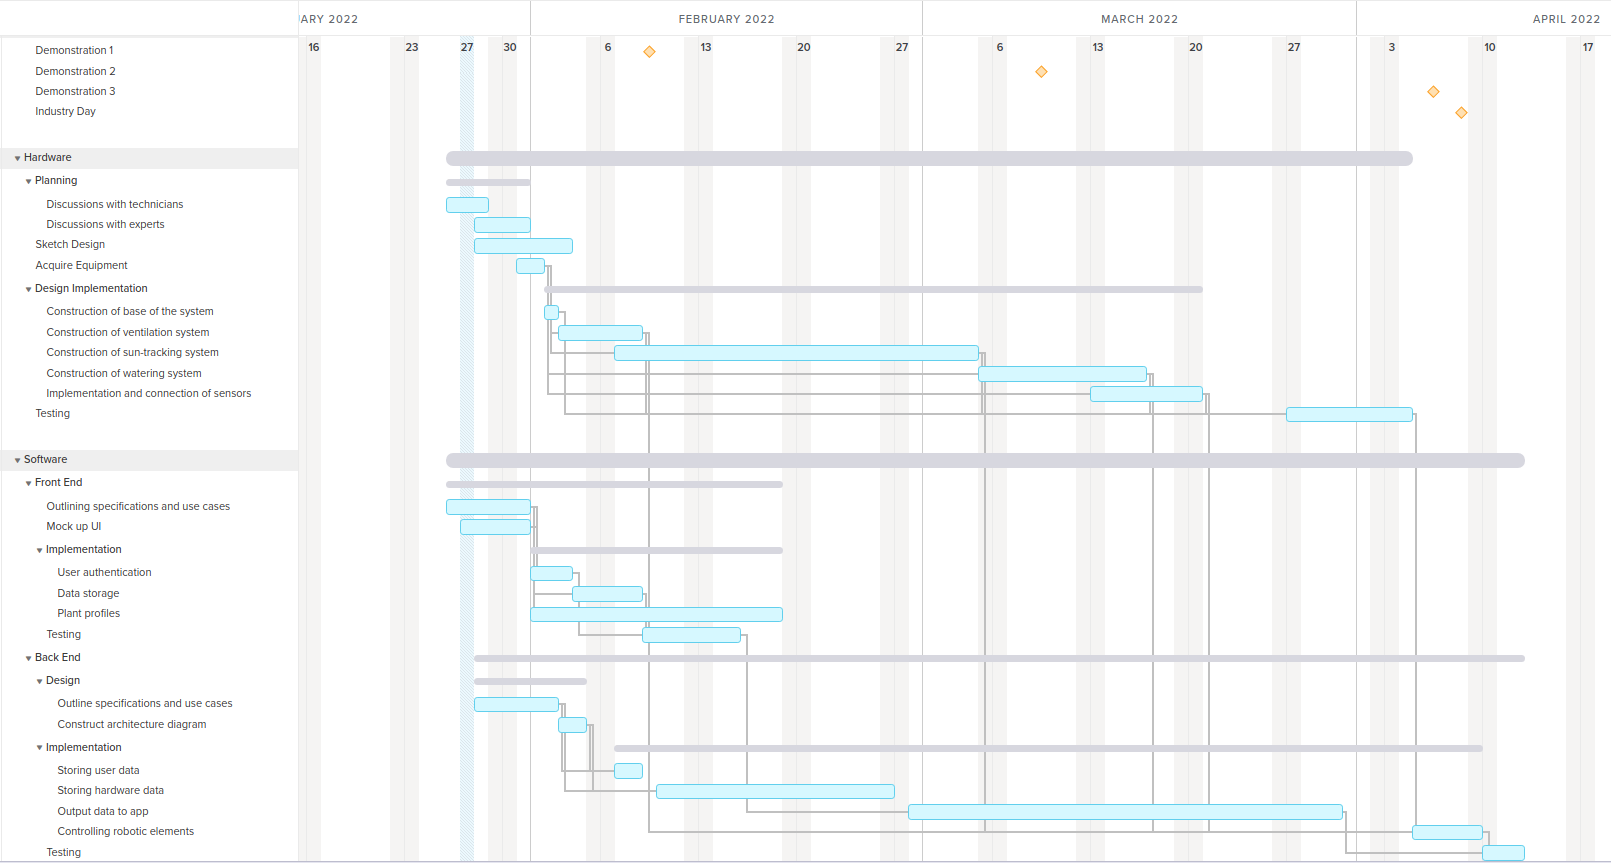
\includegraphics[width=\paperwidth]{figs/gantt.png}
    \caption{Gantt chart to visualise work breakdown structure}
    \label{fig:gantt}
\end{sidewaysfigure*}


\begin{table*}[ht]
\vskip 3mm
\begin{center}
\begin{small}
\begin{sc}
\begin{tabular}{lcp{12cm}}
\hline
\abovespace\belowspace
Demonstration & Date  & Milestone Description \\
\hline
\abovespace
Demo 1       & 09/02/2022 & Construction of the propagator base and the vent mechanism, design of website application UI and data storage, implementation of login system. \\
Demo 2       & 09/03/2022 & Implementation of sun-tracking feature and start water system if time allows, connection to and storage of hardware data stream. \\
Demo 3       & 06/04/2022 & Complete hardware construction and linking to software elements. \\
Industry Day & 08/04/2022 & Marketing strategy
\belowspace
\end{tabular}
\end{sc}
\end{small}
\caption{Milestones for the system}
\label{tab:milestones}
\end{center}
\vskip -3mm
\end{table*}


\section{Tasks}

\subsection{Subsystems}
We have agreed as a team that it would be most appropriate to split the construction of our plant care system into two broad subgroups, which are the hardware and software aspects of the design. This allows each member of the team to focus on their particular areas of interest, whilst still working with other people, and makes the division of atomic tasks clearer.

The initial development of these two subsystems is relatively independent, but they will be reliant on each other when implementing the control elements of the robotic components. To ensure that this runs smoothly we intend to continue with daily meetings as a whole group to discuss progress, obstacles, and so on.

The hardware and software subsystems will each account for approximately 50\% of the time spent on developing the product and each of these subsystems can be further subdivided into the high-level descriptions described by subsections 6.1.1 and 6.1.2. Please see the Gantt chart presented in Figure \ref{fig:gantt} for a more comprehensive and detailed overview. Moreover, it should be noted that the team members will be subdivided into the two subsystems based on the strengths and interests outlined in the Teams section, but there are possibilities for task rotations for the interested. 

\subsubsection{High-Level Overview Hardware}
The hardware division will be responsible for the physical implementation of the smart plant care system, which consists of the following areas:

\begin{enumerate}
    \item Foundation/base of the propagator (10\%)
    \item Ventilation system     (10\%)
    \item Sun-tracking system    (40\%)
    \item Watering system        (35\%)
    \item Sensor incorporation   (5\%)
\end{enumerate}

The current intention is to build these hardware components in the sequential manner described above. Even if some of the above tasks could be constructed in parallel such as the sun-tracking and the watering system, doing so would cause too much complications as the systems might interfere with each other if not fully complete. In addition, doing these demanding tasks sequentially will also allow for the exchange of ideas to facilitate production. However, it should be noted that some sensor incorporation will occur in parallel with the other tasks as they will utilise inputs from sensors.

\subsubsection{High-Level Overview Software}
The software team will be responsible for implementing the website-application that allows users to interact with the system. The following features are to be implemented:
\begin{enumerate}
    \item User Interface (40\%)
    \item API     (15\%)
    \item Database    (25\%)
    \item Data Processing        (20\%)
    \item Machine learning algorithm for optimal plant conditions (Potential Extension)
\end{enumerate}
In similarity to the hardware team, the tasks will be implemented in the order specified above. We intend on first implementing the user interface which will be user-friendly and an easy-to-use web application. This is anticipated to take a significant period of time. Linking and setting up the API will be the next challenge. Furthermore, we will then have to work closely with the hardware team to receive data from the sensors and process this data into a user-friendly format in our application. Depending on time constraints we would also like to implement machine learning features so that our system learns for future reference the best conditions for growth.

\subsection{Milestones}
The team has agreed on specific milestones in order to achieve the objectives that have been outlined in the high-level overviews and the Gantt Chart. The milestones agreed upon are presented in table \ref{tab:milestones}.

\subsection{Additional Work}
In addition to the work required for constructing the system we are also accounting for the overhead time required to attend workshops, write reports, plan demonstrations, and conduct marketing (and other ancillary) research. To ensure that these responsibilities are fairly divided amongst us, we intend to do the following:

\begin{itemize}

\item Take turns in attending workshops and then sharing this knowledge with the rest of the group,
\item Collaborating on reports so that everyone has a contribution to all sections, 
\item Sharing responsibilities for presenting at demonstrations,
\item Discussing any and all further reading regularly to account for any changes to be implemented as early as possible.

\end{itemize}

% \pagebreak


\section{Risks}

% The main risks to our project fall into three categories: ethical risks, safety concerns, and functionality concerns. We’re confident that although some of the risks are serious to the success of our project, they can mostly be mitigated.

% Firstly, we have risks pertaining to the ethics of creating what will be a relatively expensive device for schools and those from poorer urban areas – tour target demographic. Gardening, and plant growing more generally, is currently quite segregated along the lines of socio-economic background, age, and location; generally, gardeners tend to be older, more middle class, and more suburban, with gardeners on average earning 9 per cent above the average income in the UK and 67 per cent more likely to be over the age of 55. By making an expensive product we are effectively marginalising those groups who are already marginalised in gardening. If this risk is realised, we could contribute to this existing problem and fail to make the positive impact that we set out to at the beginning of this project. To mitigate this risk, we could try and ensure that our product is eligible for grants by organisations such as the Royal Horticultural Society or the National Lottery, who fund community and school gardening projects across the UK. If this grant were enough to cover a substantial amount of the product’s cost, we could have the wider impact we are looking for. This will need to be investigated further at the design stage. (https://www.rhs.org.uk/get-involved/community-gardening/resources/fundraising)

% Secondly, we have risks pertaining to the safe use of our product especially when considering one our key target audiences, young school children. Mainly, the device will need to include moving parts with considerable torque to move our plants for sun-tracking, this will mean that if a limb such as a child’s finger were caught in the mechanism it could cause significant harm. This kind of risk could lead to our product not meeting certain health and safety regulation that need to be complied with to be used in schools or other institutions. In addition to this mechanical safety risk, we have the additional risk of the use of electrical components that could, if not properly designed, shock or otherwise harm a user. All these concerns will need to be addressed at the design stage by ensuring that all mechanical parts are appropriately covered to avoid getting fingers etc. trapped in them and that they are clearly labelled when this kind of covering is not possible. In addition, we will need to test and ensure that all electrical components are appropriately shielded and that shocks aren’t possible in normal use.

% Finally, there is a significant risk that, if not designed correctly, our device could break with normal use if the watering system were to leak and spill onto sensitive electrical components. This kind of design flaw could lead to our product being unviable as it wouldn’t be able to last long enough for the cost to be substantially amortised over time for it to be a wise investment for our target audience; to mitigate this, we will need to design the watering system to fail in a way such that water wouldn’t be able to get into any of the electrically sensitive components, and able to be drained in a safe way to avoid damage to our system.

The main risks to the project fall into four categories: ethical risks, safety concerns, functionality and data privacy concerns which are outlined in the following sections. In assessing the risks, it has been concluded that although some of the risks can be harmful to the success of the project we are confident that they can largely be mitigated.

\subsection{Ethical}
The ethical concerns reside in the fact that the developed product might end up a relatively expensive device for the educational sector and those with less disposable income. Gardening, and in particular plant growing, is currently quite segregated along the dimensions of socio-economic background, age, and location. Generally, gardeners tend to be older, more middle-class, and more suburban, earning on average 9\% above the average income in the United Kingdom and 67\% more likely to be over the age of 55 (S., Danya, 2017) %\cite{Danya2017}. 

If the product turns out quite expensive then this would effectively marginalise those groups, thus further exacerbating strata already present in gardening. If this risk is realised, then this product would contribute to the existing problem and fail to make the positive impact that was intended to be achieved through this project. In order to mitigate this risk, it could be tried to ensure that our product is eligible for funding by organisations such as the Royal Horticultural Society or the National Lottery that fund community and school gardening projects across the United Kingdom (RHS, 2021b). This grant might be enough to cover a substantial amount of the product’s cost and if this is the case then the wider positive impact that was intended could be achieved. However, this will need to be investigated further at the design stage. 

\subsection{Safety}
There will be risks pertaining to the safe use of the developed product, especially when considering its interaction with school-age children that are part of the main target audience. Firstly, it should be emphasised that the device will need to include moving parts with considerable torque to move the plants for the sun-tracking feature of the design. This will mean that if a body part such as a child’s finger was caught in the mechanism then it could cause significant damage to them. This sort of risk could lead to the product not meeting certain health and safety regulations that need to be complied with in the school premises or other institutions. In addition, there is the risk of the use of electrical components that could, if not properly designed, shock or otherwise harm the user, which is especially important to consider as the product will store liquid as well. These concerns will need to be addressed at the design stage by ensuring that all the mechanical parts are appropriately covered to prevent body parts from becoming trapped in the device. Moreover, it has to be ensured that it is clearly mentioned and labeled when this sort of mechanical covering is not possible. Furthermore, it will be ensured through testing that all electrical components are properly shielded with insulated material and that shocks are not present nor possible during normal use. Safety precautions about proper handling of robot should be added to the app as users' compulsory reading.

\subsection{Functionality}
From the functional design perspective, if the foundation and base of the product are not designed correctly then the device could potentially break during normal use, especially if the watering system was to leak and spill onto sensitive electrical components. This form of design flaw could lead to the product not being viable as it would not be able to last long enough for the cost to be substantially amortised over time such that it becomes a wise investment for the target audience. In order to mitigate this, the watering system will have to be designed such that if it fails the water would not be able to get into any of the electrically sensitive components and would be able to be drained in a safe way to avoid damage to the overall system.

\subsection{Data privacy}
There will potentially be a camera component added to the project to monitor the growth of the plant and this might be a worrisome function as there could be a misuse of the camera if the product is connected to the internet and attacked by a third party. This means that data collected from all sensors should pertain the necessary confidentiality given by the user. Furthermore, people should be aware that their data will be collected and analysed to allow the user to utilise all the different functionality of the website application to ensure the best user experience possible.
% \begin{itemize}

%     \item A risk we must be aware of in our system is with the watering features of our system. Obviously having water in an electronic system can be dangerous as if it's not done correctly water could leak into the system and cause the whole thing to break. So, in order to reduce the chances of this happening the features involving water should be thoroughly tested outside of the main system before being added.
    
%     \item A serious risk is that if our product is too highly priced it could exacerbate existing barriers of entry to gardening, pricing out those who would otherwise benefit the most from the system such as state schools or people in financially depressed urban areas.
    
%     \item Another risk is that the product has too short a lifetime or is hard to maintain and repair, means that lifetime cost of ownership is increased further exacerbating the above issue.
    
%     \item Moreover, the fact that the device is robotic and electronic presents a safety risk - especially to young children, one of our target audiences. This would need to be mitigated at the design phase to ensure that the device doesn't risk trapping fingers or other limbs, and / or shocking the user.
    
%     \item As the previous concept of our product, it should track the sunshine and move, if the propagator is on a table or anything higher than the ground level, it might fall and break during moving. (I think we can solve this by limiting the area the propagator can move and slow down its speed)

%     \item Another point is that the propagator is an electricity device, we should consider how to make it be safe during use from a childproof consideration. (no good solution in my mind so far).
    
%     \item One risk is error information in individual profiles for different plant species. We know that different plants have various circadian rhythms. If our app informs the wrong message to users who are without planting experiences, it may be bad for plant growth or even cause plant death.
    
%\end{itemize}

%% Include any references in a bibliography
%\bibliographystyle{unsrt}
%\bibliography{proposal-references}

\begin{thebibliography}{}
\small
\bibitem{a} Survey: \textit{Decorating with houseplants}. \textit{Article.com}, 2020. Available at: \url{https://www.article.com/blog/survey-decorating-with-houseplants/} [Accessed 27 January 2022].

\vspace{0.2cm}

\bibitem{b} A\&M, Texas. \textit{Health and well-being benefits of plants}, Available at: \url{https://ellisonchair.tamu.edu/health-and-well-being-benefits-of-plants/} [Accessed 27 January 2022].

\vspace{0.2cm}

\bibitem{c} Han, Ke-Tsung. \textit{Influence of limitedly visible leafy indoor plants on the psychology, behaviour, and health of students at a junior high school in taiwan}. \textit{EDRA}, 41:658-692, 2008. Available at: \url{https://journals.sagepub.com/doi/10.1177/0013916508314476} [Accessed 27 January 2022].

\vspace{0.2cm}

\bibitem{d} Middleton, Karie. \textit{Leave it to the expert: Seven most difficult plants to grow in your garden}. 2018. Available at \url{https://www.gardenbuildingsdirect.co.uk/blog/seven-plants-difficult-grow/} [Accessed 27 January 2022].

\vspace{0.2cm}

\bibitem{i} RHS 2021a. \textit{Houseplants: to support human health}. [online] Available at: \url{https://www.rhs.org.uk/plants/types/houseplants/for-human-health} [Accessed 27 January 2022].

\bibitem{e} RHS. 2021b \textit{Fundraising for your community garden}. Available at: \url{https://www.rhs.org.uk/get-involved/community-gardening/resources/fundraising} [Accessed 27 January 2022].

\bibitem{f} S., Danya. \textit{What is the demographic information around people in the uk that practice home gardening?} 2017. Available at: \url{https://askwonder.com/research/demographic-information-around-people-uk-practice-home-gardening-pi77tzwyz#:~:text=Consumers\%20aged\%2045\%2D54\%20years,female\%20aged\%2055\%20and\%20older.} [Accessed 27 January 2022].

\bibitem{g} Society of Biology, 2010. \textit{The Importance of Practical Biology}: from School to Higher Education. [online] Society of Biology. Available at: \url{https://www.rsb.org.uk/images/Practical\%20Biology\%20Position\%20Paper.pdf} [Accessed 27 January 2022]. 

\bibitem{h} Sayan, H. and Mertoğlu, H., 2020. \textit{Equipment Use in Biology Teaching}. Journal of Educational Issues, [online] 6(1), pp.357-371. Available at: \url{https://www.macrothink.org/journal/index.php/jei/article/view/17042} [Accessed 27 January 2022].

\end{thebibliography}
% We can replace the links with their proper referencing later. I am just
% including them now so that we know the correspondence between what the source and the things we state.

% \begin{itemize}
    %\item 1. \url{https://www.article.com/blog/survey-decorating-with-houseplants/}
    %\item 2. \url{https://www.saps.org.uk/attachments/article/556/SSR%20September%202015%20052-056%20Jenkins.pdf}
    %\item 3. \url{https://nph.onlinelibrary.wiley.com/doi/full/10.1002/ppp3.43}
    %\item 4. \url{https://journals.sagepub.com/doi/10.1177/0013916508314476}
    %\item 5. \url{https://ellisonchair.tamu.edu/health-and-well-being-benefits-of-plants/}
    %\item 6. \url{https://askwonder.com/research/demographic-information-around-people-uk-practice-home-gardening-pi77tzwyz#:~:text=Consumers%20aged%2045%2D54%20years,female%20aged%2055%20and%20older.}
    %\item 8. \url{https://www.gardenbuildingsdirect.co.uk/blog/seven-plants-difficult-grow/}
    %\item 9. \url{https://www.kingsfund.org.uk/sites/default/files/field/field_publication_file/Gardens_and_health.pdf}
% \end{itemize}

\end{document} 

